\subsection{Documentazione}
\subsubsection{Scopo}
Lo scopo di questa sezione è di redigere e standardizzare i documenti prodotti durante tutto il ciclo di vita del software. 
Di conseguenza ci si aspetta di avere:
\begin{itemize}
\item Una struttura ben organizzata e con una facile navigabilità;
\item Una serie di norme tipografiche da rispettare.
\end{itemize}
I documenti possono essere consultati nel seguente repository di \glo{GitHub}:
\\
\url{https://github.com/qb-team/Stalker-Documentazione}.
\subsubsection{Aspettative}
Questa sezione serve a fornire degli strumenti e indicazioni comuni ai membri del gruppo per arrivare a una produzione di documentazione coesa e professionale.

\subsubsection{Descrizione}
La documentazione prodotta dal \textit{processo di documentazione} registra tutte le informazioni generate durante il ciclo di vita di un processo o un'attività.
Il \textit{processo di documentazione} deve contenere un set di attività volte a garantire la produzione, verifica e mantenimento della documentazione.

\subsubsection{Attività}

\paragraph{Implementazione del processo}
\subparagraph*{Ciclo di vita}
Ogni documento prima di essere presentato deve passare per tre stati fondamentali:
\begin{enumerate}
\item \textbf{Stesura del documento}: Creazione del documento e stesura con il linguaggio \LaTeX;
\item \textbf{Verifica del Documento}: Il documento viene assegnato ad un verificatore, il cui lavoro è controllare che il documento rispetti gli standard definiti;
\item \textbf{Approvazione del documento}: In caso la verifica risulti positiva, il documento viene consegnato al \Responsabile{} per l'approvazione al rilascio.
\end{enumerate}

\subparagraph*{Studio di Fattibilità}
\subsubsection{Studio di fattibilità}
Il \Responsabile{} ha il compito di convocare tutti i membri del gruppo \Gruppo{} per discutere le varie tematiche riguardanti i capitolati d'appalto disponibili.
Lo \SdF{} viene redatto dagli analisti, i quali devono analizzare il materiale disponibile e inoltre tenere in considerazione anche ciò che è stato discusso nelle riunioni sul tema.\\
Il documento è strutturato in più sezioni, ognuna riguardante un capitolato d'appalto.
Per ogni capitolato verranno trattati i seguenti punti:
\begin{itemize}
\item Titolo del capitolato:
	\begin{itemize}
	\item Nome del capitolato;
	\item Azienda proponente;
	\item Committenti.
	\end{itemize}
\item Descrizione del capitolato:
	\begin{itemize}
	\item Breve riassunto del prodotto da realizzare, secondo le specifiche richieste dal proponente.
	\end{itemize}
\item Prerequisiti e tecnologie coinvolte:
	\begin{itemize}
	\item Elenco delle tecnologie da utilizzare, con eventuali riferimenti per ulteriori approfondimenti o spiegazioni del contesto applicativo;
	\item In alcuni casi l'azienda proponente consiglia l'utilizzo di certe tecnologie.
	\end{itemize}
\item Vincoli:
	\begin{itemize}
	\item Richieste generali, tecniche e/o organizzative da parte dell'azienda proponente.
	\end{itemize}
\item Aspetti positivi:
	\begin{itemize}
	\item Vengono descritti gli aspetti ritenuti positivi dai membri del gruppo \Gruppo{} del capitolato.
	Possono essere considerati aspetti positivi, ad esempio, l'apprendimento di nuove tecnologie e/o linguaggi, disponibilità di contatto e collaborazione offerta dal proponente e documentazione disponibile online riguardante le tecnologie coinvolte.
	\end{itemize}
\item Aspetti critici:
	\begin{itemize}
	\item Vengono descritti gli aspetti ritenuti critici dai membri del gruppo \Gruppo{} del capitolato.
	Possono essere considerati aspetti critici, ad esempio, l'eccessiva mole di tecnologie da apprendere, i requisiti di vincolo da tenere in considerazione e la scarsa presenza di documentazione online riguardante le tecnologie coinvolte.
	\end{itemize}
\item Conclusioni:
	\begin{itemize}
	\item Valutazione finale motivata dai membri del gruppo \Gruppo{} nella quale vengono esposte le ragioni di interesse o disinteresse nella scelta o meno del capitolato.
	\end{itemize}
\end{itemize}
Tutte queste informazioni appena elencate vengono raccolte nel documento interno \glo{\SdF{}}, sottoposto al processo di \glo{verifica{}} da parte dei verificatori.
\subparagraph*{Piano di Progetto}
\documentclass[a4paper, oneside, dvipsnames, table]{article}
%openany
\usepackage{../../template/Stiletemplate}
\usepackage{hyperref}
\usepackage{fancyhdr}
\usepackage[italian]{babel}
\usepackage[raggedright]{titlesec}
\usepackage{blindtext}
\titleformat{\paragraph}[hang]{\normalfont\normalsize\bfseries}{\theparagraph}{1em}{}
\titlespacing*{\paragraph}{0pt}{3.25ex plus 1ex minus .2ex}{0.5em}

\newcommand{\Data}{2019-12-13}

\newcommand{\Titolo}{Verbale Riunione \Data}

\newcommand{\Redattori}{\MC{}}

\newcommand{\Verificatori}{\DF{}}

\newcommand{\Approvatore}{\AT{} \newline \SE{}}

\newcommand{\Distribuzione}{\VT{} \newline \CR{} \newline Gruppo \Gruppo{}}

\newcommand{\Uso}{Interno}

\newcommand{\DescrizioneDoc}{Questo documento si occupa di riportare quanto discusso nella riunione del \Data}

\newcommand{\pathimg}{../../../Utilita/Immagini/qbteam.png}

\newcommand{\Versionedoc}{1.0.0}


\begin{document}

\copertina{}
\newpage


\fancyPdP{}

\clearpage
\tableofcontents
% scritto da\AT{}
\section{Introduzione}
\subsection{Scopo del documento}
Il presente documento ha lo scopo di descrivere le strategie che il gruppo \Gruppo{} intende applicare per garantire la qualità di processo e di prodotto per l’intera durata del progetto.
Al fine di rispettare questi obiettivi vengono descritte le modalità in cui vengono effettuate la verifica e la validazione del prodotto.
In questo modo è consentita la rilevazione e correzione di problemi o incongruenze in breve tempo, senza correre il rischio di sprechi di risorse.

\subsection{Scopo generale del prodotto}
L'obiettivo del prodotto \NomeProgetto{} di \Proponente{} è la creazione di un sistema software composto di un applicativo per cellulare e di un server, con cui interagire tramite un'interfaccia utente. La necessità nasce dal bisogno di adempiere alle normative vigenti in tema di sicurezza.
Le due componenti del sistema software, applicativo e server, devono soddisfare i seguenti obiettivi rispettivamente di:
\begin{itemize}
\item Tracciare e registrare i \glo{movimenti} di un utente in un \glo{luogo di tracciamento} di un'\glo{organizzazione}, siano essi autenticati da credenziali di un'\glo{organizzazione} oppure visitatori anonimi, il tutto nel rispetto della normativa sulla privacy;
\item Poter visionare gli accessi degli utenti autenticati e visionare il numero di visitatori anonimi all'interno di un luogo.
\end{itemize}

\subsection{Glossario}
Al fine di evitare ambiguità fra i termini, e per avere chiare fra tutti gli stakeholder le terminologie utilizzate per la realizzazione del presente documento, il gruppo \Gruppo{} ha redatto un documento denominato \Glossariov{1.0.0}.
In tale documento, sono presenti tutti i termini tecnici, ambigui, specifici del progetto e scelti dai membri del gruppo con le loro relative definizioni.
Un termine presente nel \Glossariov{1.0.0} e utilizzato in questo documento viene indicato con un apice \ap{G} alla fine della parola.

\subsection{Standard di progetto}
Il gruppo \Gruppo{} ha deciso di gestire i propri processi del ciclo di vita del software adottando alcune parti dello standard \textbf{ISO/IEC 12207} come definito nelle \textit{NormeDiProgetto}; 
come modello di qualità del prodotto software si è utilizzato parte dello standard \textbf{ISO/IEC 9126} anch'esso definito nelle \textit{NormeDiProgetto}.

\subsection{Riferimenti}

\subsubsection{Normativi}
\begin{itemize}
    \item \textbf{Capitolato d'appalto C5 - Stalker}\\     
    \url{https://www.math.unipd.it/~tullio/IS-1/2019/Progetto/C5.pdf};
    \item \NdPv{1.0.0}.
    \item \textbf{ISO/IEC 12207-1995:}\\     
    \url{https://www.math.unipd.it/~tullio/IS-1/2009/Approfondimenti/ISO_12207-1995.pdf};\\
    \url{http://www.colonese.it/SviluppoSw_Standard_ISO12207.html};
    \item \textbf{ISO/IEC 9126:}\\
    \url{http://www.colonese.it/00-Manuali_Pubblicatii/07-ISO-IEC9126_v2.pdf};\\
    \url{https://en.wikipedia.org/wiki/ISO/IEC_9126};
\end{itemize}

\subsubsection{Informativi}
\begin{itemize}
    \item \textbf{Indice di Gulpease}\\
    \url{https://it.wikipedia.org/wiki/Indice_Gulpease};
    \item \textbf{Metriche di progetto}\\
    \url{https://it.wikipedia.org/wiki/Metriche_di_progetto};
    \item \textbf{Varie metriche}\\
    \url{http://torlone.dia.uniroma3.it/sistelab/annipassati/sbavaglia.pdf};
    \item \textbf{Ciclo di Deming - Plan Do Check Act}\\
    \url{https://it.wikipedia.org/wiki/Ciclo_di_Deming};
    
\end{itemize}
\clearpage
\section{Analisi dei Rischi}
La gestione dei rischi è un processo al quale il gruppo qbteam dà molto importanza. Questo perchè incorrere contro ad un rischio potrebbe equivalere al daneggiamento del progetto, sia nella sua organizzazione e sia nella sua qualità.
Quindi si cerca di fare una previsione dei problemi che si potranno verificare durante l'intero corso del progetto e ad ogni problema riscontrato si cerca una soluzione per poterlo evitare.

\subsection{Fasi della gestione dei rischi}
Il gruppo seguirà le seguenti fasi del processo di gestione dei rischi:
\begin{itemize}
	\item \textbf{Identificazione del rischio}
	\\ Questa è la prima fase del processo e ci serve per identificare i rischi che potrebbero portare a dei problemi durante l'avanzamento del progetto; 
\end{itemize}
\begin{itemize}
	\item \textbf{Analisi dei rischi}
	\\ Dopo aver individuato i rischi nella fase precedente, per ognuno di essi si valuterà la probabilità che esso si verifichi e le conseguenze negative che potrebbe portare;
\end{itemize}
\begin{itemize}
	\item \textbf{Pianificazione del rischio}
	\\ In Pianificazione del rischio si sviluppano dei piani per sapere quali rimedi bisognerà intraprendere nel momento in cui i rischi si verificano. In tale modo si riuscirà a risolvere i problemi prima che essi diventano gravi.
\end{itemize}
\begin{itemize}
	\item \textbf{Monitoraggio del rischio} 
	\\ Nell'ultima fase della gestione del rischio si verifica che le ipotesi relative ai rischi non abbiano subito delle variazioni. Quindi si cerca di valutare periodicamente la probabilità che il rischio si verifichi e i suoi possibili effetti cercando di adottare strategie migliori alla loro risoluzione.
\end{itemize}

\subsection{Tipologia del rischio}
Ci sono 6 tipi di rischi che il gruppo qtbeam terrà in considerazione. 
\\Ad ogni rischio verrà assegnato un codice identificativo:
\begin{itemize}
	\item Rischi Tecnologici [RT];
	\item Richi Organizzativi [RO];
	\item Rischi Personali [RP];
	\item Rischi dei Requisiti [RR];
	\item Rischi Strumentali [RS];
	\item Rischi di Stima [RE];
\end{itemize}

\subsection{Tabella dei rischi}
Nella seguente tabella veranno elencati i rischi che il gruppo qbteam potrebbe incontrare durante l'intero ciclo di vita del progetto.
Ogni colonna di un rischio sarà composto da:
\begin{itemize}
	\item Codice [codice del tipo + numero di occorrenze dello stesso tipo] e Nome del Rischio;
	\item Descrizione;
	\item Rilevamento;
	\item Piano di Contingenza;
\end{itemize}



{
\rowcolors{2}{grigetto}{white}
\renewcommand{\arraystretch}{1.5}
\centering
\begin{longtable}{ c c  C{4cm}  C{3cm} C{4cm}}
\rowcolor{darkblue}
\textcolor{white}{\textbf{Codice}} & \textcolor{white}{\textbf{Nome}} & \textcolor{white}{\textbf{Descrizione}} & \textcolor{white}{\textbf{Rilevamento}} & \textcolor{white}{\textbf{Probabilità e Gravità}} & \textcolor{white}{\textbf{Risoluzione}}\\	

RT1 & Inesperienza alle tecnologie & Il gruppo dovrà affrontare tecnologie mai utilizzate precedentemente e quindi servirà del tempo per poter imparare ad utilizzarle nel modo corretto & Ogni componente del gruppo sarà consapevole di saper usare una determinata tecnologia & Probabilità Alta Gravità Media & Ogni componente del gruppo che ha acquisito una certa abilità nell'utilizzo di una tecnologia, cercherà di aiutare i componenti del gruppo che hanno più difficoltà \\
		

\end{longtable}
}
\clearpage
\section{Modello di Sviluppo}
\clearpage
\section{Pianificazione}
Nella pianificazione, il responsabile suddividerà il lavoro in attività e le assegnerà a ciascun membro del team.
Lo scopo è quello di mostrare come verrà svolto il lavoro, valutare i progressi nel progetto e anticipare i problemi che potrebbero sorgere preparando così delle soluzioni a tali problemi. 
La pianificazione di progetto è stata organizzata seguendo le scadenze presenti nella sezione § 8.1 Scadenze.
Lo sviluppo del progetto è stato suddiviso nelle seguenti 4 fasi: 
\begin{itemize}
	\item Analisi;
	\item Progettazione Architetturale;
	\item Progettazione di Dettaglio e Codifica;
	\item Validazione e Collaudo;
\end{itemize}
Ogni fase sarà suddivisa in periodi più brevi all'interno dei quali verranno elencate le diverse attività che il gruppo \Gruppo{} svolgerà.


\subsection{Analisi}

\subsubsection{Periodo 1} 
Dal 2019-11-15 al 2019-11-29\\
In questo periodo, che parte dalla formazione del gruppo e termina con la scelta del capitolato C5, abbiamo affrontato le seguenti tematiche al fine di porre le basi per il lavoro che dovevamo affrontare:\\
\begin{itemize}
	\item \textbf{Discussione capitolati:} per prima cosa abbiamo studiato individualmente e in seguito discusso durante gli incontri tutti i capitolati proposti, questo ha posto le basi per la stesura del documento \SdF{} e ci ha indirizzati verso la scelta del capitolato che avremmo affrontato;
	\item \textbf{Spartizione e studio dei ruoli:} a ogni membro del gruppo è stato assegnato il ruolo che svolgerà nella fase di Analisi;
	\item \textbf{Definizione degli strumenti:} Abbiamo discusso e definito le tecnologie che avremmo usato per affrontare la fase di Analisi;
	\item \textbf{Pianificazione milestone fase di Analisi:} Abbiamo discusso e fissato delle milestone da rispettare per completare la fase di Analisi entro le scadenze imposteci.
\end{itemize}
\subsubsection{Periodo 2} 
Dal 2019-11-30 al 2019-12-31\\
Questo periodo inizia con la scelta definitiva del capitolato C5.\\
Dopo la scelta abbiamo focalizzato le risorse del gruppo sui seguenti punti:
\begin{itemize}
	\item \textbf{Normazione: }Abbiamo definito le regole per la stesura dei documenti e per l'utilizzo delle tecnologie identificate in precedenza;
	\item \textbf{Approfondimento capitolati: }Abbiamo ulteriormente discusso tutti i capitolati in modo da terminare lo studio di fattibilità e focalizzato la nostra analisi su quello scelto in modo da predisporre le basi per l'analisi dei requisiti;
	\item \textbf{Prima definizione dei casi d'uso};
	\item \textbf{Determinazione standard di qualità: }Abbiamo definito le nostre strategie per garantire la qualità di processo e di prodotto;
	\item \textbf{Verifica: }Verifica dell'andamento del team in relazione alle tempistiche e allo svolgimento dei compiti assegnati.
\end{itemize}
\subsubsection{Periodo 3}
 Dal 2020-01-01 al 2020-01-14\\
 Questo periodo si estende fino alla data ultima di consegna per affrontare la revisione dei requisiti a cui il nostro gruppo ha deciso di partecipare.\\
 \begin{itemize}
	\item \textbf{Normazione: }Ulteriori approfondimenti alle regole per la stesura dei documenti e per l'utilizzo delle tecnologie;
	\item \textbf{Approfondimento delle tecnologie: }Abbiamo ampliato le nostre conoscenze sulle tecnologie richieste dal capitolato per essere svolto;
	\item \textbf{Analisi dei requisiti: } Studio dei requisiti e raffinamento dei casi d'uso;
	\item \textbf{Pianificazione attività: }Pianificazione del lavoro da svolgere nelle fasi successive a quella di Analisi;
	\item \textbf{Verifica: }Verifica dell'andamento del team in relazione alle tempistiche e allo svolgimento dei compiti assegnati.

 \end{itemize}
\subsubsection{Periodo 4} 
Dal 2020-01-15 al 2020-01-20\\
In questo periodo che parte dalla consegna dei documenti per la revisione dei requisiti alla presentazione pubblica della proposta il gruppo consolida il lavoro svolto in vista delle successive fasi e della discussione per la quale serve una presentazione;
\begin{itemize}
	\item \textbf{Consolidamento:} Ogni membro si prende del tempo per ripassare tutto il lavoro svolto e per studiare il necessario per affrontare al meglio le fasi successive;
	\item \textbf{Preparazione per la Revisione dei Requisiti:} Il gruppo produce il materiale necessario da esporre alla presentazione pubblica della nostra proposta.
\end{itemize}

	\newpage
	% Inizia la pagina orientata orizzontalmente
	\begin{landscape}
	 % Ora la pagina e' in orizzontale!
	\subsubsection{Diagramma di Gantt delle attività}
	\pagestyle{empty}
	\begin{figure}[h]
		
		\begin{center}	
			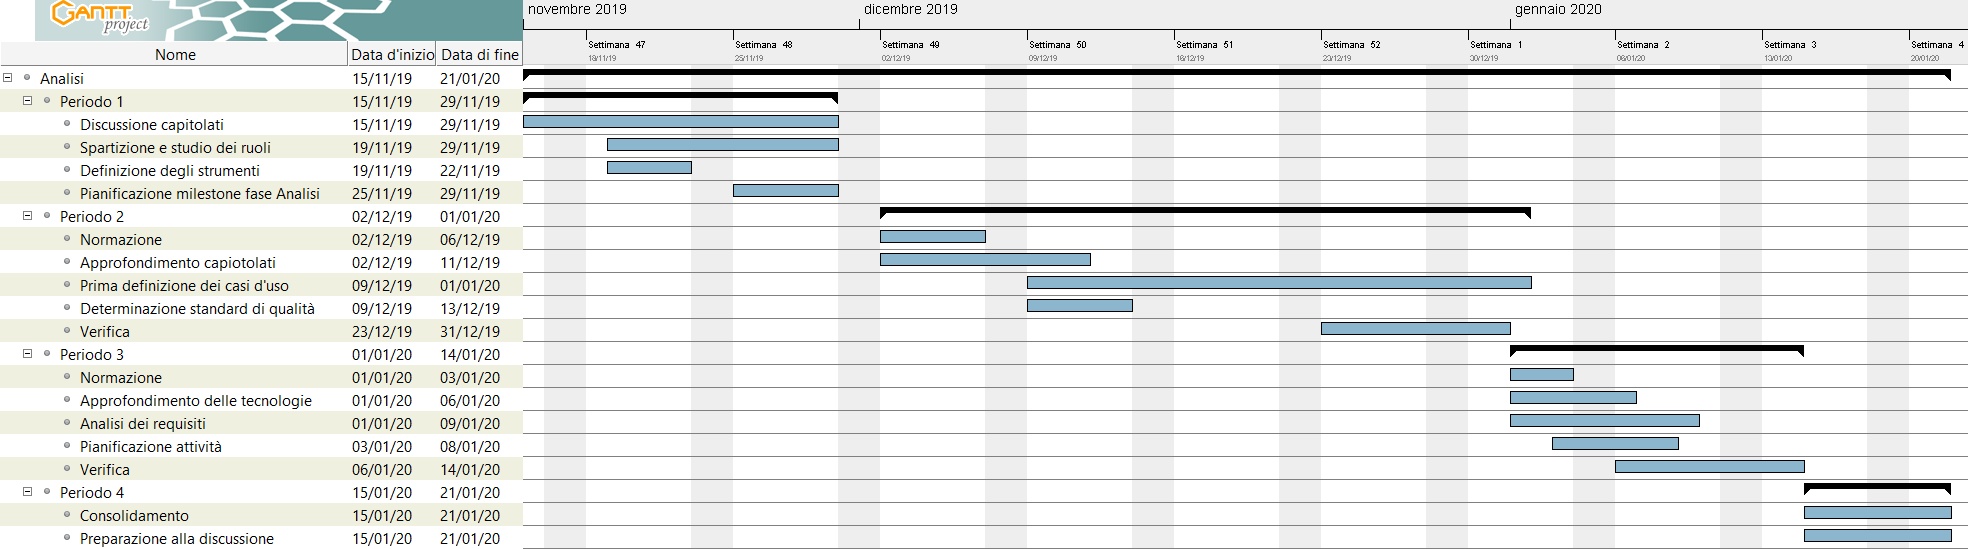
\includegraphics[scale=0.50]{Sezioni/DiagrammiGantt/Analisi.png}
		\end{center}
	\caption{Diagramma di Gantt delle attività di Analisi}
	\end{figure}
	 \end{landscape}

\clearpage
\subsection{Progettazione Architetturale}
Periodo: dal 2020-01-22 al 2020-03-15.
\\Inizia al termine dell'Analisi dei Requisiti e finisce con la data di consegna della Revisione di Progettazione.
\\In questa fase viene definita una soluzione architetturale in modo da soddisfare i requisiti individuati nel periodo di Analisi dei Requisiti.

\subsubsection{Periodo 1} 
Dal 2020-01-22 al 2020-02-11
\begin{itemize}
	\item \textbf{Normazione};
	\item \textbf{Analisi dei requisiti};
	\item \textbf{Pianificazione attività};
	\item \textbf{Approfondimento delle tecnologie};
	\item \textbf{Verifica}.
\end{itemize}
\subsubsection{Periodo 2} 
Dal 2020-02-12 al 2020-03-08
\begin{itemize}
	\item \textbf{Studio delle tecnologie:} IAAS Kubernetes\ap{G} o PaaS\ap{G}, Openshift\ap{G} o Rancher\ap{G}, LDAP\ap{G} e GPS\ap{G};
	\item \textbf{Normazione};
	\item \textbf{Miglioramento standard di qualità};
	\item \textbf{Technology Baseline\ap{G}:} redazione della Technology baseline;
	\item \textbf{Proof of Concept\ap{G}:} rappresentazione della Baseline\ap{G};
	\item \textbf{Codifica:} viene codificato il Proof of Concept;
	\item \textbf{Verifica}.
\end{itemize}
\subsubsection{Periodo 3} 
Dal 2020-03-09 al 2020-03-15
\begin{itemize}
	\item \textbf{Consolidamento};
	\item \textbf{Preparazione per la Revisione di Progettazione Architetturale}.
\end{itemize}

\newpage
% Inizia la pagina orientata orizzontalmente
\begin{landscape}
	% Ora la pagina e' in orizzontale!
	\subsubsection{Diagramma di Gantt delle attività}
	\pagestyle{empty}
	\begin{figure}[h]
		
		\begin{center}	
			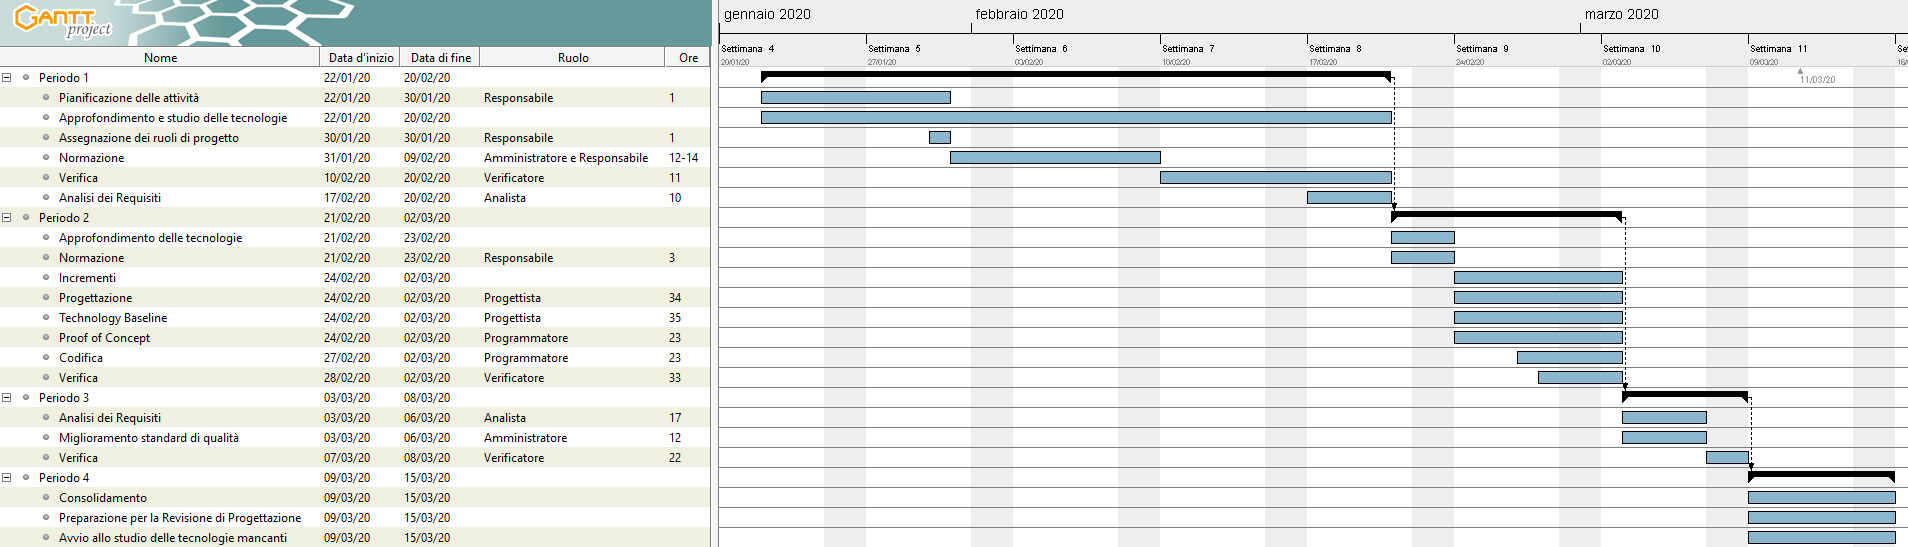
\includegraphics[scale=1.6]{Sezioni/DiagrammiGantt/ProgettazioneArchitetturale.png}
		\end{center}
	\caption{Diagramma di Gantt delle attività di Progettazione}	
	\end{figure}
\end{landscape}

\subsection{Progettazione di Dettaglio e Codifica}
Dal 2020-03-16 al 2020-04-19\\
Inizia al termine della Progettazione Architetturale e finisce con la data di consegna della Revisione di Qualifica.\\
In questa fase si definisce nel dettaglio e si implementa l'architettura logica costruita nella fase di Progettazione Architetturale.\\


\subsubsection{Periodo 1} 
Dal 2020-03-16 al 2020-03-27\\
\begin{itemize}
	\item \textbf{Approfondimento delle tecnologie};
	\item \textbf{Normazione};
	\item \textbf{Pianificazione delle attività};
	\item \textbf{Progettazione};
	\item \textbf{Codifica:} Implementazione dei requisiti di base identificati per ottenere un sistema stabile;
	\item \textbf{Manuali:} Stesura manuale utente e manuale manutentore in relazione alle funzionalità di base del sistema.
\end{itemize}
\subsubsection{Periodo 2} 
Dal 2020-03-28 al 2020-04-08\\
\begin{itemize}
	\item \textbf{Implementazione della Product Baseline:} seguendo le specifiche della Technology Baseline;
	\item \textbf{Codifica incrementale:} Aggiunta di requisiti al sistema tramite incrementi;
	\item \textbf{Incremento e verifica:} Verifiche ed eventuali aggiunte al lavoro svolto in precedenza;
	\item \textbf{Manuali:} Aggiunta nel manuale utente e nel manuale manutentore delle funzionalità inserite incrementalmente nel sistema;
\end{itemize}
\subsubsection{Periodo 3}
Dal 2020-04-09 al 2020-04-12\\
\begin{itemize}
	\item \textbf{Primo rilascio del prodotto};
	\item \textbf{Verifica:} Verifica dell'andamento del team in relazione alle tempistiche e allo svolgimento dei compiti assegnati;
\end{itemize}
\subsubsection{Periodo 4} 
Dal 2020-04-13 al 2020-04-19\\
\begin{itemize}
	\item \textbf{Consolidamento};
	\item \textbf{Preparazione per la Revisione di Qualifica}.
\end{itemize}

\newpage
% Inizia la pagina orientata orizzontalmente
\begin{landscape}
	% Ora la pagina e' in orizzontale!
	\subsubsection{Diagramma di Gantt delle attività}
	\pagestyle{empty}
	\begin{figure}[h]
			
		\begin{center}	
				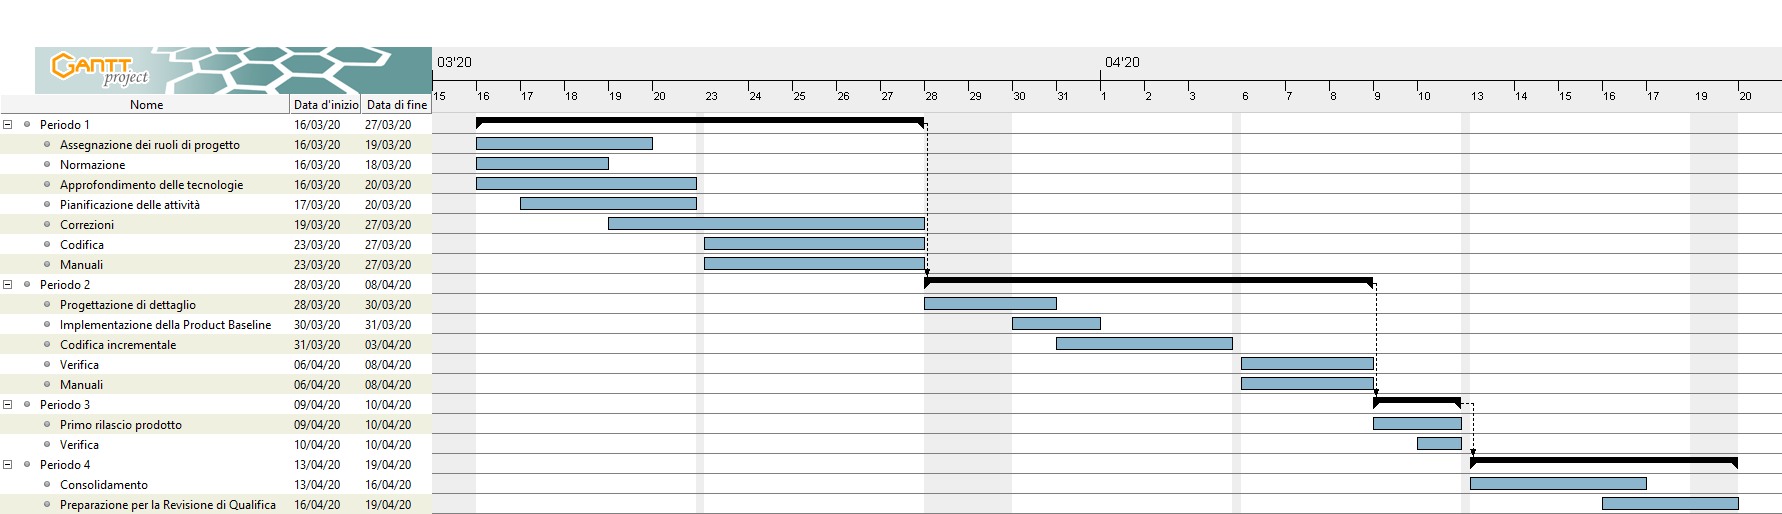
\includegraphics[scale=0.5]{Sezioni/DiagrammiGantt/ProgettazioneDiDettaglio.png}	
		\end{center}
	\caption{Diagramma di Gantt delle attività di Progettazione di Dettaglio e Codifica}	
	\end{figure}
\end{landscape}

\subsection{Validazione e Collaudo}
Inizia al termine della Progettazione di Dettaglio e Codifica e finisce con la data di consegna della Revisione di Accettazione.
\\In questo fase vengono definite le attività che servono per verificare che il prodotto corrisponde a quello desiderato dal cliente.
\subsubsection{Periodo 1} 
Dal 2020-04-21 al 2020-04-28
\begin{itemize}
	\item \textbf{Normazione};
	\item \textbf{Analisi dei requisiti};
	\item \textbf{Pianificazione attività};
	\item \textbf{Verifica}.
\end{itemize}
\subsubsection{Periodo 2} 
Dal 2020-04-29 al 2020-05-10
\begin{itemize}
	\item \textbf{Codifica:} verrà eseguito l'ultimo versionamento del prodotto;
	\item \textbf{Verifica:} verrà accertato che le esecuzioni delle attività siano esenti da errori;
	\item \textbf{Validazione:} verrà verificato se il prodotto realizzato sia conforme alle attese;
	\item \textbf{Scrittura dei manuali:} verrà eseguito il secondo versionamento del manuale Utente e del manuale Manutentore;
	\item \textbf{Collaudo:} vengono eseguiti gli ultimi test sul prodotto per verificare se le funzionalità rispettano i risultati attesi.
\end{itemize}
\subsubsection{Periodo 3} 
Dal 2020-05-11 al 2020-05-17
\begin{itemize}
	\item \textbf{Preparazione per la Revisione di Accettazione}.
\end{itemize}


\newpage
% Inizia la pagina orientata orizzontalmente
\begin{landscape}
	% Ora la pagina e' in orizzontale!
	\subsubsection{Diagramma di Gantt delle attività}
	\pagestyle{empty}
	\begin{figure}[h]
		
		\begin{center}	
			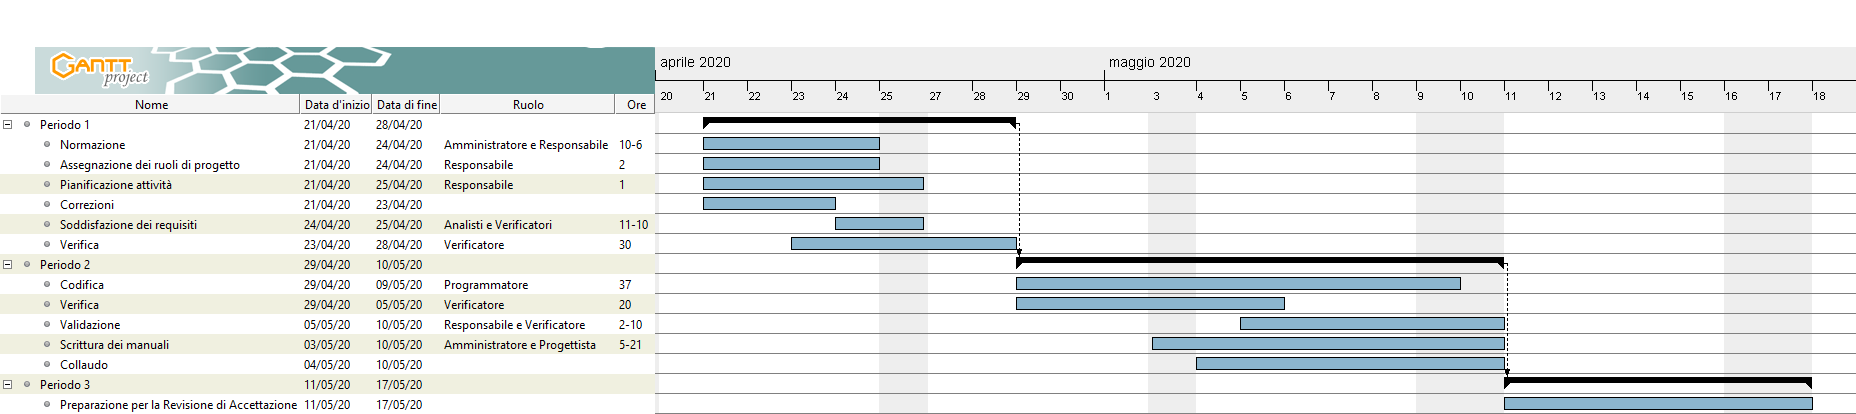
\includegraphics[scale=1.6]{Sezioni/DiagrammiGantt/Validazione.png}
		\end{center}
	\caption{Diagramma di Gantt delle attività di Validazione e Collaudo}	
	\end{figure}
\end{landscape}
\clearpage
\section{Preventivo}
Sigle identificative per i ruoli indicati nelle tabelle e nei grafici:
\begin{itemize}
    \item RE: Responsabile;
    \item AM: Amministratore;
    \item AN: Analista;
    \item PT: Progettista;
    \item PR: Programmatore;
    \item VE: Verificatore.
\end{itemize}
{
	
\rowcolors{2}{grigetto}{white}
\renewcommand{\arraystretch}{2}
\begin{table}[h!]
\centering
\caption{Tabella con i costi per ogni ruolo}
\begin{longtable}{ C{3cm} C{3cm}}
\rowcolor{darkblue}
	\textcolor{white}{\textbf{Ruolo}} & 
	\textcolor{white}{\textbf{Costo per ora espresso in euro}}\\	
			
			Responsabile & 30\\
			Amministratore & 20\\
			Analista & 25\\
			Progettista & 22\\
			Programmatore & 15\\
			Verificatore & 15\\
			
		\end{longtable}
		
	\end{table}

}

\clearpage
\subsection{Fase di Analisi}
\subsubsection{Divisione Oraria}

La seguente tabella rappresenta la distribuzione oraria dei ruoli per ogni componente del gruppo:
\rowcolors{2}{grigetto}{white}
\renewcommand{\arraystretch}{2}
\begin{table}[h!]
\centering
\caption{Tabella della divisione oraria di Analisi}	
\begin{longtable} { C{4cm} C{1cm} C{1cm} C{1cm} C{1cm} C{1cm} C{1cm} C{3cm}}

\rowcolor{darkblue}
	\textcolor{white}{\textbf{Membro del gruppo}} & 
	\textcolor{white}{\textbf{RE}} & 
	\textcolor{white}{\textbf{AM}} & 
	\textcolor{white}{\textbf{AN}} & 
	\textcolor{white}{\textbf{PT}} & 
	\textcolor{white}{\textbf{PR}} & 
	\textcolor{white}{\textbf{VE}} & 
	\textcolor{white}{\textbf{Ore complessive}}\\	
\endhead        

        \MC{}     &  & 7 & 12 &  & & 11 & 30 \\
		\LD{}       &  & 5 & 16 &  &  & 9 & 30 \\
        \CE{}     &  &  & 21 &  &  & 9 & 30 \\
        \SE{}       & 15 & 2 & 8  &  &  & 5 & 30 \\
        \PF{}       &  &  & 21 &  &  & 9 & 30 \\
        \DF{}      &  & 7 & 16 &  &  & 7 & 30 \\
        \BR{}     &  & 5 & 11 &  &  & 14 & 30 \\
       \AT{}      & 4 & 12 & 9  &  &  & 5 & 30 \\
        \textbf{Ore totali ruolo} & 19 & 38 & 114 &  &  & 69 & 240 \\
        
\end{longtable}
\end{table}
\newline
La quantità di ore che ciascun componente del gruppo ha svolto per ogni ruolo viene rappresentata nel seguente istogramma:
\begin{figure}[h]
	\centering
	\caption{Disposizione ore per ruolo di ciascun componente della fase di Analisi}
	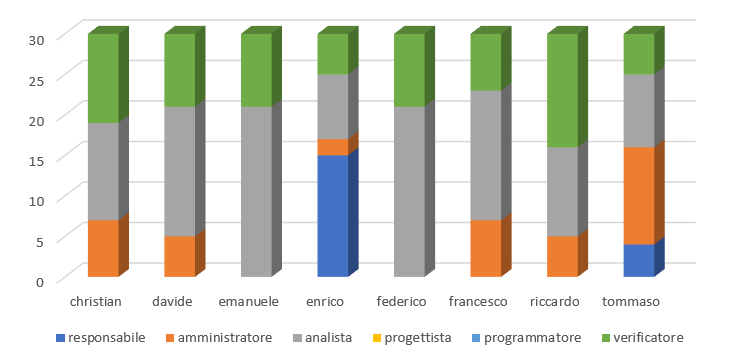
\includegraphics[scale=2.35]{sezioni/Istogrammi/IstogrammaAnalisi.png}
	
\end{figure}

\clearpage
\subsubsection{Costo Risultante}
La seguente tabella rappresenta per ogni ruolo le ore totali investite e il corrispondente costo in euro:
{
\rowcolors{2}{grigetto}{white}
\renewcommand{\arraystretch}{2}
\begin{table}[h]
\centering
\caption{Tabella del costo risultante di Analisi}
\begin{longtable}{ C{3cm} C{2cm} C{4cm}}
\rowcolor{darkblue}
	\textcolor{white}{\textbf{Ruolo}} & 
	\textcolor{white}{\textbf{Totale ore}} & 
	\textcolor{white}{\textbf{Costo ruolo in euro}}\\	
\endhead

        Responsabile & 19 & 570\\
        Amministratore & 38 & 760\\
        Analista & 114 & 2850 \\
        Progettista & 0 & 0 \\
        Programmatore & 0 & 0 \\
        Verificatore & 69 & 1035 \\
        \textbf{Totale} & 240 & 5215 \\
		
	\end{longtable}
\end{table}
}


La quantità di ore totali per ciascun ruolo viene rappresentata nel seguente areogramma:
\begin{figure}[h]
\centering
	\caption{Suddivisione ore per ruolo della fase di Analisi}
	
	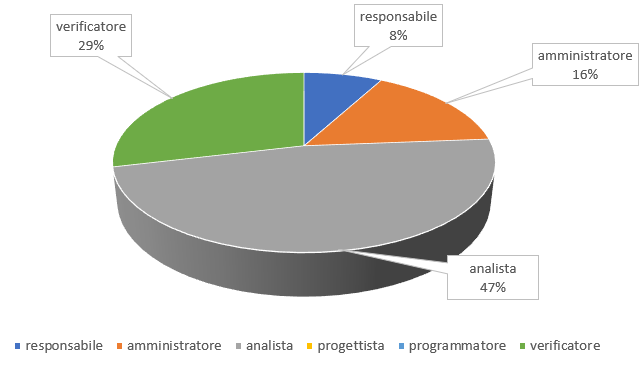
\includegraphics[scale=2.85]{sezioni/Aerogrammi/AerogrammaAnalisi.png}
\end{figure}
\clearpage

\subsection{Progettazione Architetturale}

\subsubsection{Divisione Oraria}
La seguente tabella rappresenta la distribuzione oraria dei ruoli per ogni componente del gruppo:
{
\rowcolors{2}{grigetto}{white}
\renewcommand{\arraystretch}{2}
\begin{table}[h]
\caption{Tabella della divisione oraria della Progettazione Architetturale}
\begin{longtable}{ C{5cm} C{1cm} C{1cm} C{1cm} C{1cm} C{1cm} C{1cm} C{3cm}}
\rowcolor{darkblue}
	\textcolor{white}{\textbf{Nome membro del gruppo}} & 
	\textcolor{white}{\textbf{RE}} & 
	\textcolor{white}{\textbf{AM}} & 
	\textcolor{white}{\textbf{AN}} & 
	\textcolor{white}{\textbf{PT}} & 
	\textcolor{white}{\textbf{PR}} & 
	\textcolor{white}{\textbf{VE}} & 
	\textcolor{white}{\textbf{Ore complessive}}\\	
	\endhead
        
    \MC{} & 5 & & & 14 & 10 & 4 & 33\\
    \LD{} & 8 & & & 18 & & 7 & 33 \\
    \CE{} & & 8 & & 10 & 5 & 6 & 29 \\
    \SE{} & & 10 & 6 & 10 & & 6 & 32 \\
    \PF{} & & 6 & & 5 & 7 & 13 &  31\\
    \DF{} & & & 13 & 5 & 7 & 6 & 31 \\
    \BR{} & 6 & & & & 17 & 8 & 31\\
   \AT{} & & & 8 & 7 & & 16 & 31\\
	\textbf{Ore totali ruolo} & 19 & 24 & 27 & 69 & 46 & 66 & 251\\
		
	\end{longtable}
\end{table}
}

La suddivisione delle ore svolte da ciascun componente del gruppo per ogni ruolo viene rappresentata nel seguente istogramma:

\begin{figure}[h!]
	\centering
	\caption{Disposizione ore per ruolo di ciascun componente della fase di Progettazione Architetturale}
	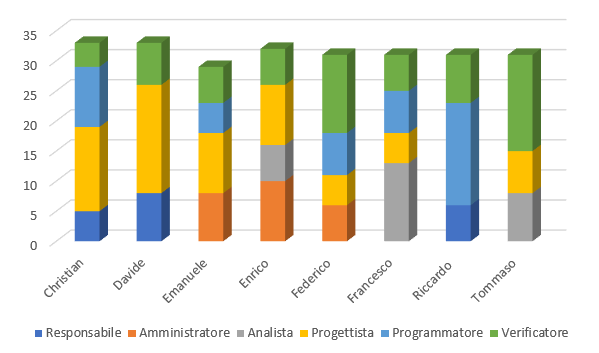
\includegraphics[scale=3]{sezioni/Istogrammi/IstogrammaProgettArchitetturale.png}
\end{figure}


\subsubsection{Costo Risultante}
La seguente tabella rappresenta per ogni ruolo le ore totali investite e il corrispondente costo in euro:
{
\rowcolors{2}{grigetto}{white}
\renewcommand{\arraystretch}{2}
\centering
\begin{table}[h]
\caption{Tabella del costo risultante della Progettazione Architetturale}
\begin{longtable}{ C{3cm} C{2cm} C{4cm}}
\rowcolor{darkblue}
	\textcolor{white}{\textbf{Ruolo}} & 
	\textcolor{white}{\textbf{Totale ore}} & 
	\textcolor{white}{\textbf{Costo ruolo in euro}}\\	
\endhead
        
        Responsabile & 19 & 570 \\
        Amministratore & 24 & 480 \\
        Analista & 27 & 675 \\
        Progettista & 69 & 1518 \\
        Programmatore & 46 & 690 \\
        Verificatore & 66 & 990 \\
        \textbf{Totale} & 251 & 4923 \\	
        	
	\end{longtable}
\end{table}
}

La suddivisione della quantità di ore totali per ciascun ruolo viene rappresentata nel seguente areogramma:

\begin{figure}[h]
	\centering
	\caption{Suddivisione ore per ruolo della fase di Progettazione Architetturale}
	
	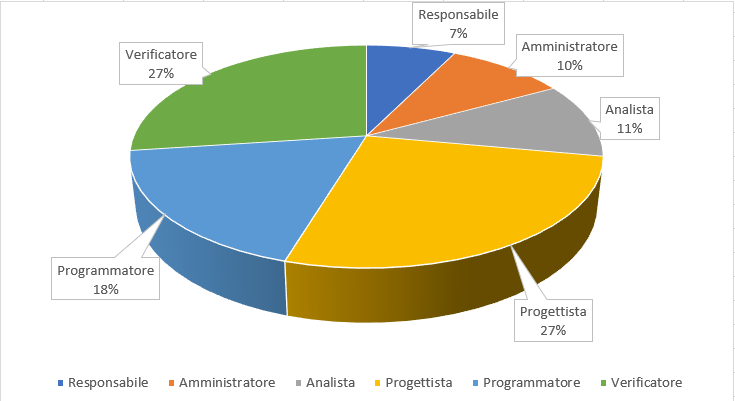
\includegraphics[scale=1.9]{sezioni/Aerogrammi/AerogrammaProgettArchitetturale.png}
\end{figure}

\clearpage
\subsection{Progettazione di dettaglio e codifica}

\subsubsection{Divisione Oraria}
La seguente tabella rappresenta la distribuzione oraria dei ruoli per ogni componente del gruppo:
{
	\rowcolors{2}{grigetto}{white}
	\renewcommand{\arraystretch}{2}
	\begin{table}[h]
	\caption{Tabella della divisione oraria della Progettazione di Dettaglio e Codifica}
	
\begin{longtable}{ C{5cm} C{1cm} C{1cm} C{1cm} C{1cm} C{1cm} C{1cm} C{3cm}}
\rowcolor{darkblue}
	\textcolor{white}{\textbf{Nome membro del gruppo}} & 
	\textcolor{white}{\textbf{RE}} & 
	\textcolor{white}{\textbf{AM}} & 
	\textcolor{white}{\textbf{AN}} & 
	\textcolor{white}{\textbf{PT}} & 
	\textcolor{white}{\textbf{PR}} & 
	\textcolor{white}{\textbf{VE}} & 
	\textcolor{white}{\textbf{Ore complessive}}\\
\endhead	
        
        \MC{} & & 10 & & 12 & 15 & 10 & 47\\
        \LD{} & 6 & & & 10 & 15 & 16 & 47\\
        \CE{} & & 5 & & 13 & 16 & 13 & 47 \\
        \SE{} & & 4 & & 11 & 18 & 14 & 47\\
        \PF{} & & 8 & & 8 & 19 & 12 & 47\\
        \DF{} & 10 & & & 7 & 17 & 13 & 47\\
        \BR{} & & 3 & & 12 & 19 & 13 & 47\\
       \AT{} & 10 & & & 10 & 17 & 10 & 47 \\
        \textbf{Ore totali ruolo} & 26 & 30 & & 83 & 136 & 101 & 376\\
		
	\end{longtable}
\end{table}
}
\newline
La suddivisione di quante ore, ciascun componente del gruppo, ha svolto per ogni ruolo viene rappresentata nel seguente istogramma:



\begin{figure}[h!]
\centering
\caption{Disposizione ore per ruolo di ciascun componente della fase di Progettazione di Dettaglio e Codifica}
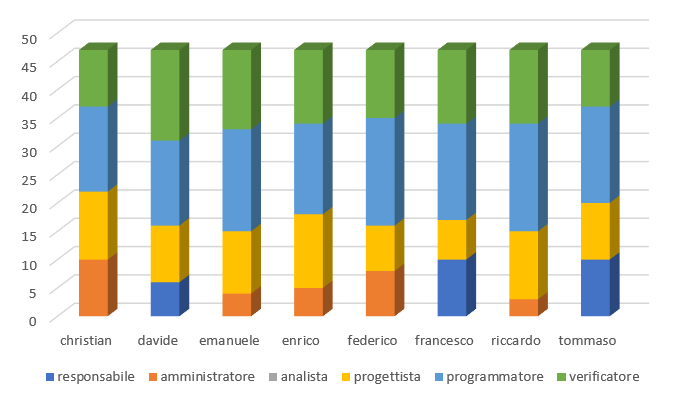
\includegraphics[scale=2.5]{sezioni/Istogrammi/IstogrammaDiDettaglio.png}
\end{figure}

\subsubsection{Costo Risultante}
La seguente tabella rappresenta, per ruolo, le ore totali investite e il corrispondente costo in euro:
{
\rowcolors{2}{grigetto}{white}
\renewcommand{\arraystretch}{2}
\begin{table}[h]
\centering
\caption{Tabella del costo risultante della Programmazione di Dettaglio e Codifica}
\begin{longtable}{ C{3cm} C{2cm} C{4cm}}
\rowcolor{darkblue}
	\textcolor{white}{\textbf{Ruolo}} & 
	\textcolor{white}{\textbf{Totale ore}} & 
	\textcolor{white}{\textbf{Costo ruolo in euro}}\\	
\endhead
        
        Responsabile & 26 & 780 \\
        Amministratore & 30 & 600 \\
        Analista & 0 & 0 \\
        Progettista & 83 & 1826 \\
        Programmatore & 136 & 2040 \\
        Verificatore & 101 & 1515\\
        \textbf{Totale} & 376 & 6761 \\
		
	\end{longtable}
\end{table}
}

La suddivisione della quantità di ore totali per ciascun ruolo viene rappresentata nel seguente areogramma:

\begin{figure}[h]
	\centering
	\caption{Suddivisione ore per ruolo della fase di Progettazione di Dettaglio e Codifica}
	
	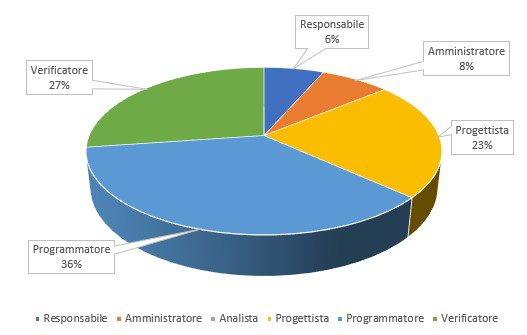
\includegraphics[scale=2.8]{sezioni/Aerogrammi/AerogrammaDiDettaglio.png}
\end{figure}

\clearpage
\subsection{Validazione e Collaudo}

\subsubsection{Divisione Oraria}
La seguente tabella rappresenta la distribuzione oraria dei ruoli per ogni componente del gruppo:
{
	\rowcolors{2}{grigetto}{white}
	\renewcommand{\arraystretch}{2}
	\begin{table}[h]
		\caption{Tabella della divisione oraria di Validazione e Collaudo}

	\begin{longtable}{ C{5cm} C{1cm} C{1cm} C{1cm} C{1cm} C{1cm} C{1cm} C{3cm}}
		\rowcolor{darkblue}
		\textcolor{white}{\textbf{Nome membro del gruppo}} & \textcolor{white}{\textbf{RE}} & \textcolor{white}{\textbf{AM}} & \textcolor{white}{\textbf{AN}} & \textcolor{white}{\textbf{PT}} & \textcolor{white}{\textbf{PR}} & \textcolor{white}{\textbf{VE}} & \textcolor{white}{\textbf{Ore complessive}}\\	
        
        \MC{} & & & 7 & & 4 & 8 & 19\\
        \LD{} & & 4 & & 5 & & 10 & 19\\
        \CE{} & 5 & & & & 6 & 12 & 23\\ 
        \SE{} & & & & 6 & 5 & 9 & 20 \\
        \PF{} & 6 & & & & 7 & 8 & 21\\
        \DF{} & & 6 & & & 9 & 6 & 21\\
        \BR{} & & 5 & & & 6 & 10 & 21\\
       \AT{} & & & 4 & 10 & & 7 & 21\\
        \textbf{Ore totali ruolo} & 11 & 15 & 11 & 21 & 37 & 70 & 165\\
		
	\end{longtable}
\end{table}
}


La suddivisione delle ore svolte da ciascun componente del gruppo per ogni ruolo viene rappresentata nel seguente istogramma:

\begin{figure}[h!]
	\centering
	\caption{Disposizione ore per ruolo di ciascun componente della fase di Validazione e Collaudo}
	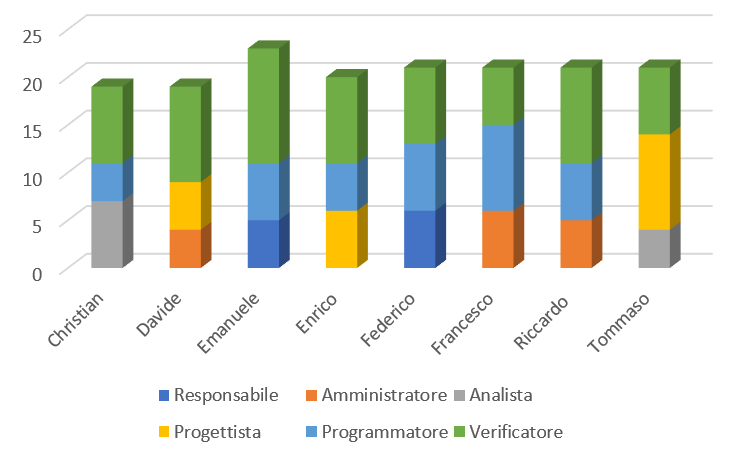
\includegraphics[scale=2.5]{sezioni/Istogrammi/IstogrammaValidazione.png}
\end{figure}

\subsubsection{Costo Risultante}
La seguente tabella rappresenta rappresenta per ogni ruolo le ore totali investite e il corrispondente costo in euro:
{
	\rowcolors{2}{grigetto}{white}
	\renewcommand{\arraystretch}{2}
\begin{table}[h!]
	\caption{Tabella del costo risultante di Validazione e Collaudo}
	\begin{longtable}	{ C{3cm} C{2cm} C{4cm}}

		\rowcolor{darkblue}
		\textcolor{white}{\textbf{Ruolo}} & \textcolor{white}{\textbf{Totale ore}} & \textcolor{white}{\textbf{Costo ruolo in euro}}\\	
        
        Responsabile & 11 & 330\\
        Amministratore & 15 & 300 \\
        Analista & 11 & 275\\
        Progettista & 21 & 462\\
        Programmatore & 37 & 555\\
        Verificatore & 70 & 1050\\
        \textbf{Totale} & 169 & 2972\
	
	\end{longtable}
\end{table}
	
}

La suddivisione della quantità di ore totali per ciascun ruolo viene rappresentata nel seguente areogramma:

\begin{figure}[h]
	\centering
	\caption{Suddivisione ore per ruolo della fase di Validazione e Collaudo}
	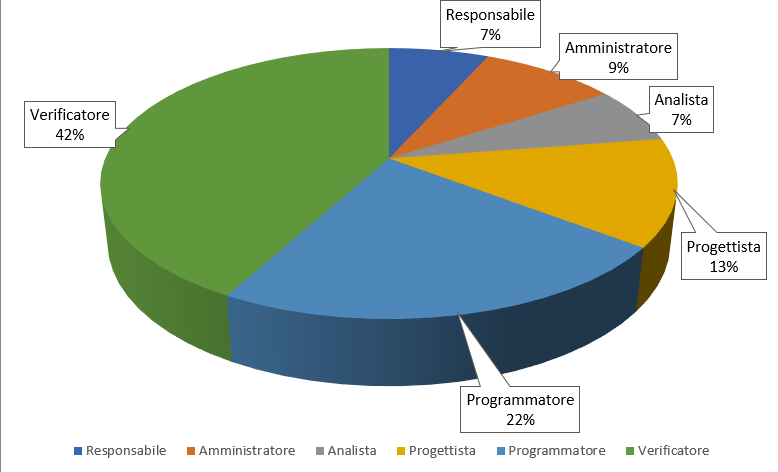
\includegraphics[scale=2.5]{sezioni/Aerogrammi/AerogrammaValidazione.png}
\end{figure}


\clearpage
\subsection{Preventivo finale} 
Nel preventivo riportiamo la spesa totale che il committente dovrà affrontare, derivata dal totale delle ore rendicontate e preventivate nelle fasi di Progettazione Architetturale, Progettazione di Dettaglio e Codifica, Validazione e Collaudo.

\subsubsection{Divisione oraria complessiva} 
Nella seguente tabella viene mostrata la distribuzione oraria dei ruoli per ogni componente del gruppo:
{
	\rowcolors{2}{grigetto}{white}
	\renewcommand{\arraystretch}{2}
\begin{table}[h]
		\caption{Tabella della divisione oraria complessiva}

	\begin{longtable}{ C{5cm} C{1cm} C{1cm} C{1cm} C{1cm} C{1cm} C{1cm} C{3cm}}
		\rowcolor{darkblue}
		\textcolor{white}{\textbf{Nome membro del gruppo}} & \textcolor{white}{\textbf{RE}} & \textcolor{white}{\textbf{AM}} & \textcolor{white}{\textbf{AN}} & \textcolor{white}{\textbf{PT}} & \textcolor{white}{\textbf{PR}} & \textcolor{white}{\textbf{VE}} & \textcolor{white}{\textbf{Ore complessive}}\\	
        
        \MC{} & 5 & 10 & 7 & 26 & 29 & 22 & 99 \\
        \LD{} & 14 & 4 & & 33 & 15 & 33 & 99\\
        \CE{} & 5 & 13 & & 23 & 27 & 31 & 99 \\
        \SE{} & & 14 & 6 & 27 & 23 & 29 & 99\\
        \PF{} & 6 & 14 & & 13 & 33 & 33 & 99\\
        \DF{} & 10 & 6 & 13 & 12 & 33 & 25 & 99 \\
        \BR{} & 6 & 8 & & 12 & 42 & 31 & 99 \\
       \AT{} & 10 & & 12 & 27 & 17 & 33 & 99 \\
        \textbf{Ore totali ruolo} & 56 & 69 & 38 & 173 & 219 & 237 &  792 \\

	\end{longtable}
\end{table}
}
\subsubsection{Costo complessivo per ruolo}
Nella seguente tabella viene illustrato il monte ore risultante per ogni ruolo con il costo ad esso associato:
{
	\rowcolors{2}{grigetto}{white}
	\renewcommand{\arraystretch}{2}
\begin{table}[h]
	\caption{Tabella del costo complessivo per ruolo}
	\begin{longtable}{ C{3cm} C{2cm} C{4cm}}
		\rowcolor{darkblue}
		\textcolor{white}{\textbf{Ruolo}} & \textcolor{white}{\textbf{Totale ore}} & \textcolor{white}{\textbf{Costo ruolo in euro}}\\	
        
        Responsabile & 56 &  1680\\
        Amministratore & 69 & 1380 \\
        Analista & 38 & 950 \\
        Progettista & 173 & 3806 \\
        Programmatore & 219 & 3285 \\
        Verificatore & 237 & 3555 \\
        	
	\end{longtable}
\end{table}
}

\subsubsection{Costo complessivo}
Nella seguente tabella vengono riportati i costi complessivi delle varie fasi e infine l'importo proposto da \Gruppo{} per la realizzazione del progetto \NomeProgetto{}:\\
{
	\rowcolors{2}{grigetto}{white}
	\renewcommand{\arraystretch}{2}

	\begin{table}[h]
	\caption{Tabella del costo complessivo}
	\begin{longtable}{ C{5cm} C{5cm}}
		\rowcolor{darkblue}
		\textcolor{white}{\textbf{Fase}} & \textcolor{white}{\textbf{Costo Fase}}\\	
		
		Progettazione Architetturale & 4923 \\
		Progettazione di Dettaglio e Codifica & 6761 \\
		Validazione e Collaudo & 2972 \\
		\textbf{Totale} & 14656\\
		
	\end{longtable}
\end{table}
}




\clearpage


\end{document}
\subparagraph*{Piano di Qualifica}
Nel documento \PdQ{} verrà descritta la strategia utilizzata dai verificatori per effettuare nel miglior modo possibile la verifica e la validazione di tutti i documenti prodotti da \Gruppo{}.

Lo scopo nel dirigere il \PdQ{} è quello di:
\begin{itemize}
	\item Illustrare come si intende gestire la qualità di processo e di prodotto;
	\item Elencare le varie metriche definite per aderire alle definizioni degli standard;
	\item Elencare i test per verificare la corretta soddisfazione dei requisiti del prodotto software.
\end{itemize}

La qualità di processo e la qualità di prodotto sono due aspetti chiaramente coordinati, ma vengono gestiti separatamente. \\ \\
Le sezioni principali del documento sono le seguenti:
\begin{itemize}
    \item \textbf{Qualità di processo:} Sezione dove vengono elencate le metriche inerenti ai \glo{processi};
    \item \textbf{Qualità di prodotto:} Sezione dove vengono elencate le metriche inerenti al prodotto;
    \item \textbf{Strategia di testing:} Sezione dove viene elencato il piano di testing delle componenti e del sistema software nel suo complesso;
\end{itemize}


\subparagraph*{Analisi dei Requisiti}

L'analisi dei requisiti è un'attività che avviene prima di quella di sviluppo.\\
Il documento \AdR{}, redatto dagli analisti, ha come scopo i seguenti punti:
\begin{itemize}
\item Definire lo scopo del prodotto da realizzare;
\item Fissare le funzionalità del progetto concordate col proponente;
\item Fornire ai progettisti riferimenti precisi ed affidabili per la progettazione dell'architettura software;
\item Definire una base per integrare i raffinamenti che permettono un miglioramento continuo del prodotto e del \glo{processo} di sviluppo;
\item Fornire ai verificatori dei riferimenti per l’attività di controllo;
\item Fornire una stima del quantitativo di lavoro da svolgere per tracciare una stima dei costi. 
\end{itemize}

L'obiettivo è quello di creare un documento formale contenente tutti i \glo{requisiti} richiesti e concordati col proponente.\\
Deve essere possibile fare riferimento a quanto redatto nel documento \AdR{} qualora sorgessero incomprensioni e dubbi al momento del collaudo del prodotto.

\subparagraph*{Verbali}

I verbali vengono redatti per tenere traccia delle decisioni prese negli incontri sia interni che esterni, in modo che ogni membro in caso non possa presenziare ad un incontro possa ritrovare le decisioni e aggiornarsi sui temi discussi.

\subparagraph*{Glossario}

Il Glossario raccoglie tutte le parole che riteniamo debbano essere disambiguate o contestualizzate nell'ambito del progetto per offrire una lettura che sia il meno possibile confusionaria.

\subparagraph*{Manuale Utente}
Lo scopo del Manuale Utente è di fornire delle spiegazioni semplici sull'utilizzo del sistema \NomeProgetto{} realizzato dal gruppo \Gruppo{}.\\
Il gruppo, dopo essersi confrontato e avendo analizzato come negli ultimi tempi vengano prodotti i manuali utenti degli altri software, ha deciso di non realizzare un documento nello stesso formato degli altri documenti di progetto: non viene quindi realizzato un file PDF in \LaTeX{} contenenti le istruzioni per utilizzare il sistema.
Si è deciso invece di realizzare un sito web, disponibile e visitabile da tutti i dispositivi con una connessione a internet (quindi non solo per PC) puntando molto sui contenuti multimediali invece di quelli testuali.
Il sito web è formato dalle seguenti pagine principali:
\begin{itemize}
    \item Introduzione: Pagina in cui viene introdotto al lettore lo scopo e le funzionalità offerte da \NomeProgetto{};
    \item Funzionalità (Sezione di App utenti e Web-app amministratori): Pagine in cui vengono mostrate le funzionalità dell'app (sezione §2.1 del sito) e della web-app (sezione §3.1 del sito), diviso in piccole sezioni monotematiche che presentano un breve testo contestualizzante, delle immagini e un breve video in cui viene illustrato l'utilizzo della funzionalità;
    \item Installazione (Sezione di App utenti e Web-app amministratori): Attualmente non disponibile, sono delle pagine in cui viene indicato, sempre con contenuti misti multimediali e testuali, come installare nel proprio smartphone e/o tablet l'applicazione per utenti e come utilizzare e/o installare la web-app per amministratori.
\end{itemize}

Il sito web in questione è accessibile presso questo link: \href{https://stalker-manuale-utente.readthedocs.io/}{https://stalker-manuale-utente.readthedocs.io/}.

\subparagraph*{Manuale Manutentore}
Lo scopo del Manuale Manutentore di fornire delle spiegazioni dettagliate su come è possibile sviluppare nuove funzionalità per tutte e tre le componenti del sistema \NomeProgetto{} realizzato dal gruppo \Gruppo{}.\\
Come per il Manuale Utente, si è deciso di realizzare un sito web al posto di un documento PDF. A maggior ragione, è diventata ormai prassi per il software e per le librerie, ancor di più quelli open source (tra cui il nostro), realizzare siti web comodamente navigabili in cui consultare la documentazione del codice sorgente.
Oltre al codice sorgente, nel Manuale Manutentore realizzato dal gruppo vi sono anche le spiegazioni sulle scelte architetturali e i vari diagrammi UML di classi, package e sequenza.
Il sito web è formato dalle seguenti sezioni principali:
\begin{itemize}
    \item Introduzione: Pagina in cui viene introdotto al lettore lo scopo e le funzionalità offerte da \NomeProgetto{};
    \item App utenti: Sezione in cui viene illustrato come l'app utenti è composta;
    \item Web-app amministratori: Sezione in cui viene illustrato come la web-app amministratori è composta;
    \item Backend: Sezione in cui viene illustrato come il backend è composto;
    \item REST API: Sezione in cui viene illustrato come le REST API possono essere utilizzate (sezione scritta in lingua inglese per raggiungere un pubblico di sviluppatori maggiore).
\end{itemize}

Ciascuna delle sezioni App utenti, Web-app amministratori e Backend, è composta
\begin{itemize}
    \item Introduzione: Pagina in cui vengono introdotte le funzionalità offerte da ciascuna delle componenti del sistema \NomeProgetto{}, specificatamente di quelle della sezione a cui fanno riferimento;
    \item Requisiti e installazione: Pagina in cui viene indicato, passo dopo passo, a uno sviluppatore esterno (o interno) al gruppo ciò che è necessario e cosa fare per poter sviluppare o effettuare attività di manutenzione nelle componenti software del sistema;
    \item Estendibilità: Pagina in cui viene indicato quali sono, oltre all'attività di manutenzione del codice già esistente, le possibilità di estensione e modifica (più o meno retro-compatibili) del sistema;
    \item Architettura: Pagina in cui vengono illustrate le scelte architetturali della app, web-app e backend;
    \item Diagrammi dei package, classi, sequenza: Pagine in cui vengono illustrate le scelte di progettazione di dettaglio delle componenti dell'architettura di ciascuna delle parti che compongono il sistema Stalker.
\end{itemize}

La sezione REST API invece, è formata dalle seguenti pagine e sezioni:
\begin{itemize}
    \item Introduction: Pagina in cui viene introdotto gli scopi delle REST API di \NomeProgetto{};
    \item Overview: Pagina in cui viene mostrata la lista di tutte le API accessibili da un client HTTP per utilizzare le funzionalità di \NomeProgetto{};
    \item Model: Sezione composta dalle pagine che mostrano in dettaglio come sono composte le entità del sistema \NomeProgetto{};
    \item Api: Sezione composta dalle pagine che mostrano in dettaglio gli end-point accessibili per implementare all'interno di un applicativo software le funzionalità offerte dal sistema \NomeProgetto{}.
\end{itemize}

Il sito web in questione è accessibile presso questo link: \href{https://stalker-manuale-manutentore.readthedocs.io/}{https://stalker-manuale-manutentore.readthedocs.io/}.

\paragraph*{Progettazione e Sviluppo}

\subparagraph*{Template e struttura dei documenti}
È presente un template per i documenti, realizzato anch'esso in \LaTeX{}, per standardizzare e velocizzare la stesura della documentazione.
Ogni documento che viene redatto deve includere al suo interno il file di stile Stiletemplate.sty presente nella cartella Utilita/.
Il template fornisce i seguenti comandi:
\begin{itemize}
\item \textbf{\textbackslash copertina\{\}}: Da inserire all'inizio del documento, ne inserisce la prima pagina (o copertina);
\item \textbf{\textbackslash fancydoc\{\}}: Da inserire dopo l'indice, inserisce l'intestazione e il piè di pagina del documento. Va utilizzato in ogni documento, ad eccezione dei verbali;
\item \textbf{\textbackslash fancyverbale\{\}}: Da inserire dopo l'indice, inserisce l'intestazione e il piè di pagina del verbale. Da utilizzare solamente nei verbali.
\end{itemize}

Ogni documento è caratterizzato da una struttura che dovrà seguire obbligatoriamente.
Di seguito viene elencato, per ogni sezione del documento, le sue caratteristiche e la sua posizione.

\subparagraph*{Prima pagina - Copertina} 
\begin{itemize}
\item \textbf{Logo del gruppo}: Il logo viene posizionato al centro della pagina, in alto;
\item \textbf{Titolo del documento}: Indica il nome del documento ed è posizionato sotto al logo del gruppo;
\item \textbf{Informazioni gruppo}: Nome del gruppo (\Gruppo{}) e del capitolato, seguiti subito dopo dall'e-mail del gruppo; 
\item \textbf{Informazioni documento}: Tabella posizionata al centro della pagina contenente le seguenti informazioni sul documento:
\begin{itemize}
\item Versione;
\item Approvatori;
\item Redattori;
\item Verificatori;
\item Uso;
\item Distribuzione.
\end{itemize}
\item \textbf{Descrizione documento}: Breve descrizione relativa al documento posizionata in fondo alla pagina, centrata.
\end{itemize}
\subparagraph*{Registro delle modifiche}
Tabella contenente diverse informazioni sul ciclo di vita del documento, composta come segue:
\begin{itemize}
\item Versione;
\item Data;
\item Nominativo;
\item Ruolo;
\item Descrizione.
\end{itemize}
Questa tabella non deve rispettare la norma definita in "Elementi grafici", poiché non deve presentare una didascalia.

\subparagraph*{Indice}
Contiene i titoli di tutte le sezioni e sottosezioni del documento, rendendo più facile la navigazione.
Se sono presenti tabelle o immagini all'interno del documento, esse possono essere riepilogate in un indice separato, se ritenuto necessario.

\subparagraph*{Riferimenti}
Tutti i riferimenti bibliografici, normativi ed informativi, vengono inseriti in ogni documento in cui siano necessari come ultima sezione del documento, sotto forma di elenco puntato.

\subparagraph*{Intestazione - Piè di pagina}
Il contenuto del documento è posto tra intestazione e il piè di pagina:

\begin{itemize}
\item In alto a sinistra è presente il logo del gruppo \Gruppo{};
\item In alto una linea orizzontale separa l’intestazione dal contenuto;
\item In basso a sinistra è presente il titolo del documento;
\item In basso a destra è presente il numero della pagina;
\item In basso una linea orizzontale separa il piè di pagina dal contenuto.
\end{itemize}

\subparagraph*{Elementi grafici}
\begin{itemize}
\item \textbf{Tabelle}: Centrate, con la didascalia posizionata al di sopra di esse;
\item \textbf{Diagrammi}: Centrati, con la didascalia posizionata al di sotto di essi;
\item \textbf{Immagini}: Centrate, con la didascalia posizionata al di sotto di esse.
\end{itemize}

\subparagraph*{Stile del testo}
\begin{itemize}
    \item \textbf{Grassetto}:
    \begin{itemize}
        \item Utilizzato per evidenziare le voci di un elenco puntato, che vengono descritte in loco;
        \item Parole ritenute particolarmente importanti in un testo;
        \item Termini del documento \Glossario{};
        \item Codici identificativi, quando introdotti per la prima volta.
    \end{itemize}
    \item \textit{Corsivo}:
    \begin{itemize}
        \item Nome del capitolato;
        \item Nome del proponente;
        \item Nome del gruppo.
    \end{itemize}
    \item \textcolor{blue}{Link ipertestuali}: Tutti i link ipertestuali devono essere di colore blu.
\end{itemize}

\subparagraph*{Glossario}
Ogni termine di un documento che contiene una definizione nel \Glossario{} viene identificato nel seguente modo:
\begin{center}
    \glo{termine}
\end{center}

\subparagraph*{Data}
Si è deciso di seguire uno dei formati più diffusi per la rappresentazione della data:
\begin{center}
\textbf{YYYY-MM-DD}
\end{center}
in cui \textbf{YYYY} rappresenta l'anno, \textbf{MM} il mese e \textbf{DD} il giorno.
\subparagraph*{Elenchi puntati/numerati}
Ogni voce di un elenco ordinato o numerato comincia con la lettera maiuscola e termina con punto e virgola (\textbf{";"}) , tranne per l'ultimo elemento dell'elenco che termina con un punto fermo (\textbf{"."}).
Nel caso di elenchi che definiscono un termine:
\begin{itemize}
    \item Il termine deve essere in grassetto;
    \item Il termine deve essere seguito da due punti (\textbf{":"});
    \item La definizione del termine inizia con la lettera maiuscola.
\end{itemize}

\subparagraph*{Nomenclatura dei documenti}
I nomi di file (escludendo l'estensione) e cartelle sono scritti usando la convenzione "\glo{Camel Case}".
I file della documentazione prodotti avranno i seguenti nomi:
\begin{itemize}
    \item \textbf{AnalisiDeiRequisiti.pdf}: Contenente il documento \AdR{};
    \item \textbf{PianoDiProgetto.pdf}: Contenente il documento \PdP{};
    \item \textbf{PianoDiQualifica.pdf}: Contenente il documento \PdQ{};
    \item \textbf{NormeDiProgetto.pdf}: Contenente il documento \NdP{};
    \item \textbf{StudioDiFattibilita.pdf}: Contenente il documento \SdF{}.
\end{itemize}
I file dei verbali, esterni e interni, avranno i seguenti nomi:
\begin{itemize}
    \item \textbf{VI\_[YYYY]\_[MM]\_[DD].pdf}: Contenente il verbale interno del [YYYY]-[MM]-[DD];
    \item \textbf{VE\_[YYYY]\_[MM]\_[DD].pdf}: Contenente il verbale esterno del [YYYY]-[MM]-[DD].
\end{itemize}
con:
\begin{itemize}
    \item \textbf{[YYYY]} L'anno in cui si è tenuto l'\glo{incontro formale};
    \item \textbf{[MM]} Il mese in cui si è tenuto l'\glo{incontro formale};
    \item \textbf{[DD]} Il giorno in cui si è tenuto l'\glo{incontro formale}.
\end{itemize}

\subparagraph*{Tabelle nei documenti}
Le tabelle utilizzate nei documenti si differenziano sostanzialmente dalla loro struttura e dal colore.
Le tabelle con intestazione di colore:
\begin{itemize}
    \item \textcolor{rossoep}{\textbf{Rosso}}: Sono solamente le tabelle del "Registro delle modifiche";
    \item \textcolor{darkblue}{\textbf{Blu}}: Sono tutte le altre tabelle.
\end{itemize}
Le intestazioni delle tabelle devono ripetersi in ogni pagina, qualora si dovessero spezzare per mancanza di spazio.

\subsubsection{Metriche}

\paragraph{Indice di Gulpease}
\begin{itemize}
	\item \textbf{Codice:} MPC6
	\item \textbf{Descrizione:} È l'indice di leggibilità di un determinato testo. Calcola la lunghezza delle parole e delle frasi rispetto al numero totale delle lettere. Il valore è un intero da 0 a 100; se esso è inferiore a 80 sarà difficile da leggere per chi ha la licenza elementare, mentre se è inferiore a 40 sarà difficili da leggere per chi ha un diploma superiore;
	\item \textbf{Processo di riferimento:} Documentazione;
	\item \textbf{Sigla:} $IG$
	\item \textbf{Formula:} $$IG = 89 + {\frac{300 \; \cdot \; |frasi| \; - \; 10 \; \cdot \; |lettere|}{|parole|}}$$
	\item \textbf{Strumenti utilizzati:} \url{https://farfalla-project.org/readability_static/}
\end{itemize}

\subsubsection{Strumenti}
\paragraph*{\LaTeX}
Per quanto riguarda la stesura dei documenti (eccetto i manuali) il gruppo ha scelto di utilizzare il linguaggio \LaTeX{}, il quale consente una migliore qualità tipografica rispetto ai normali software di videoscrittura, ma soprattutto facilita il versionamento e la suddivisione in parti di un documento.

\paragraph*{Linguaggio UML}
Per la realizzazione dei diagrammi dei casi d'uso, delle classi, dei package, delle attività e delle sequenze viene utilizzato il linguaggio di modellazione \textbf{UML}, in particolare la versione v2.0 dello standard.

\paragraph*{Markdown e Mkdocs}
Per quanto riguarda la stesura dei manuali il gruppo ha scelto di utilizzare il linguaggio Markdown attraverso lo strumento Mkdocs, il quale consente di realizzare un sito web di documentazione in modo veramente facile e veloce, con risultati molto soddisfacenti. Come per \LaTeX{}, facilita il versionamento e la suddivisione in parti di un documento.

\paragraph*{Read the Docs}
Piattaforma online in cui il gruppo rende visitabile i due manuali, utente e sviluppatore, e con cui rende pubblico anche l'Allegato Tecnico per la revisione agile della Product Baseline.

\paragraph*{Editor \LaTeX}
Per quanto riguarda gli editor per l'utilizzo e la scrittura di \LaTeX{} vengono scelti come ufficiali:
\begin{itemize}
	\item \href{https://www.xm1math.net/texmaker/}{Texmaker}, che include editor e supporto alla correzione ortografica;
	\item \href{https://code.visualstudio.com/}{Visual Studio Code}, insieme ai plugin \href{https://github.com/James-Yu/LaTeX-Workshop}{LaTeX Workshop} (per il supporto a \LaTeX) e \href{https://github.com/bartosz-antosik/vscode-spellright}{Spell Right} (per il supporto alla correzione ortografica).
\end{itemize}
I file di \LaTeX{} (file \textbf{.tex}), per generare file PDF distribuibili, devono essere compilati.
Per \LaTeX{} sono disponibili parecchi compilatori, ma avendo definito come ufficiali i soli editor TexStudio e Visual Studio Code,
i compilatori e strumenti necessari per la compilazione sono:
\begin{itemize}
    \item \textbf{MiKTeX}: Disponibile a \href{https://miktex.org/}{questo indirizzo}, se si sceglie l'utilizzo dell'editor Texmaker;
    \item \textbf{TeX Live}: Disponibile a \href{https://www.tug.org/texlive/}{questo indirizzo}, se si sceglie l'utilizzo dell'editor Visual Studio Code (nota: è una distribuzione completa di \LaTeX, quindi offre anche strumenti che possono non essere utili ai fini del progetto);
    \item \textbf{Perl}: Disponibile a \href{http://strawberryperl.com/}{questo indirizzo} per sistemi Windows, mentre, seguendo la guida di \href{https://learn.perl.org/installing/unix_linux.html}{quest'altro} per sistemi Unix/Linux, se si sceglie l'utilizzo dell'editor Visual Studio Code.
\end{itemize}
Per compilare un file \textbf{.tex} e generare un file PDF corretto deve essere invocato tre volte il comando \textbf{pdflatex $nomeFile$}, dove $nomeFile$ è il percorso ad un file con estensione \textbf{.tex} contenente al suo interno le istruzioni:
\begin{itemize}
    \item \textbackslash begin\{document\};
    \item \textbackslash end\{document\}.
\end{itemize}
Questi file hanno sempre il nome del documento che producono, con le convenzioni di nomenclatura indicate nelle \NdP{}.

\paragraph*{UML}
Per realizzare tutti i diagrammi in UML vengono utilizzati i software \href{https://draw.io}{Draw.io} e \href{http://staruml.io/}{StarUML}, entrambi disponibile come applicazione desktop, mentre Draw.io è anche disponibile come applicazione web, permettendo la collaborazione in tempo reale.
Draw.io permette sia di salvare i file di lavoro per poterli modificare, sia di esportarli.
Il salvataggio dei file di lavoro, con Draw.io, può avvenire in file in formato:
\begin{itemize}
    \item \textbf{XML}: Il file ha estensione \textbf{.xml};
    \item \textbf{Draw.io}: Il file ha estensione \textbf{.drawio}.
\end{itemize}
Il salvataggio delle immagini da includere nei documenti deve essere in formato \textbf{PNG}, con estensione \textbf{.png}, ed esportata (con Draw.io) con i seguenti parametri:
\begin{itemize}
    \item \textbf{Spessore bordo}: 20;
    \item \textbf{DPI}: 400dpi;
    \item \textbf{Sfondo}: Non trasparente (spunta rimossa).
\end{itemize}
Le seguenti impostazioni di esportazioni si trovano in File $\rightarrow$ Esporta come $\rightarrow$ Avanzate\dots; il nome del file e lo zoom, così come profondità e altezza, sono indifferenti.
